\documentclass[%
	corpo=11pt,
    twoside,
    stile=classica,
    oldstyle,
    tipotesi=custom,
    greek,
    evenboxes,
]{toptesi}
%%%%%%%%%%%%%%%%%%%%%%%%%%%%%%%%%%%%%%%%%%%%%%%%%%%%

%% for code
\usepackage{listings}

\usepackage[utf8]{inputenc}
\usepackage[T1]{fontenc}
\usepackage{lmodern}

\usepackage{hyperref}
\hypersetup{%
    pdfpagemode={UseOutlines},
    bookmarksopen,
    pdfstartview={FitH},
    colorlinks,
    linkcolor={black},
    citecolor={black},
    urlcolor={black}
  }

%%%%%%% use PDFLATEX 

\usepackage{geometry} %for the margins
\newcommand\fillin[1][4cm]{\makebox[#1]{\dotfill}} %for the dotted line in the frontispiace

\usepackage{dcolumn}
\newcolumntype{d}{D{.}{.}{-1} } %to vetical align numbers in tables, along the decimal dot

\usepackage{amsmath}

\usepackage[square,numbers]{natbib} % for the bibliography
\bibliographystyle{unsrtnat}


%%%%%%% Local definitions
\newtheorem{osservazione}{Osservazione}% Standard LaTeX
\newtheorem{observation}{Observation}% Standard LaTeX


%% for notes
\usepackage{blindtext}

\usepackage[most]{tcolorbox}

\makeatletter
\NewDocumentCommand{\mynote}{+O{}+m}{%
  \begingroup
  \tcbset{%
    noteshift/.store in=\mynote@shift,
    noteshift=1.5cm
  }
  \begin{tcolorbox}[nobeforeafter,
    enhanced,
    sharp corners,
    toprule=1pt,
    bottomrule=1pt,
    leftrule=0pt,
    rightrule=0pt,
    colback=yellow!20,
    #1,
    left skip=\mynote@shift,
    right skip=\mynote@shift,
    overlay={\node[right] (mynotenode) at ([xshift=-\mynote@shift]frame.west) {\textbf{Note:}} ;},
    ]
    #2
  \end{tcolorbox}
  \endgroup
  }
\makeatother

%%%%%%%%%%%%%%%%%%%%%%%%%%%%%%%%%%%%%%%%%%%%%%%%
%%%%%%%%%%%%%%%%%%%%%%%%%%%%%%%%%%%%%%%%%%%%%%%%



\begin{document}\errorcontextlines=9
\english

\begin{titlepage}
\newgeometry{left=1cm,right=1cm,top=3cm,bottom=3.5cm}  %specific margins for this page

\begin{center}

{\huge POLITECNICO DI TORINO}\\[1.5cm]
\textbf{Master degree\\in Computer engineering}\\[3cm]
%\textbf{Corso di Laurea Magistrale\\in Ingegneria Matematica}\\[3cm]

{\Large GPU programming - project report}\\[1cm]
%{\Large Tesi di Laurea Magistrale}\\[0.5cm]
\textbf{\LARGE Parallelization of a JPEG decompression library on a CUDA GPGPU }\\[2cm]

\includegraphics[width=0.2\textwidth]{./Pictures/logo_polito_2021.jpg}
\vspace{4cm}


\begin{minipage}{0.85\textwidth}
\begin{flushleft}\large
\textbf{Candidate}\\
Lorenzo Chiola s287911\\

%\textit{firma dei relatori} \hfill \textit{firma del candidato}\\[0.35cm]
%\fillin\ \hfill \\
%\fillin\ \hfill \\
%\fillin\ \hfill \fillin
\end{flushleft}
\end{minipage}

\vfill

Academic Year 2022-2023
\end{center}

\restoregeometry %restor default margins 

\end{titlepage} %the frontispiece

%%%%%%% Dedication
%\ifclassica%
%{\begin{dedica}
%    A mio padre

%    \textdagger\ A mio nonno Pino
%\end{dedica}}
%%%%%%% 

\sommario%summary
%Here goes the abstrat of your thesis
Application of CUDA Parallel Computing to the JPEG decompression algorithm, in the form of the already existing NanoJPEG library. The resulting program is tested on an NVidia Jetson Nano GPU board, showing a significant performance increase on images bigger than one megapixel.

%%%%%%%%%%%%%%%%%%%%%%%%%%%%%%%%%%%%%%%%%%%%%%%%
%%%%%%%%%%%%%%%%%%%%%%%%%%%%%%%%%%%%%%%%%%%%%%%%

%\ringraziamenti%acknowledgements
%Acknowledge the people you love and/or work with
%I candidati ringraziano vivamente il Granduca di Toscana per i mezzi messi loro a disposizione, ed il signor Von Braun, assistente del prof.~Albert Einstein, per le informazioni riservate che egli ha gentilmente fornito loro, e per le utili discussioni che hanno permesso ai candidati di evitare di riscoprire l'acqua calda.

%%%%%%%%%%%%%%%%%%%%%%%%%%%%%%%%%%%%%%%%%%%%%%%%
%%%%%%%%%%%%%%%%%%%%%%%%%%%%%%%%%%%%%%%%%%%%%%%%

\tablespagetrue\figurespagetrue%to include the list of tables
%and the list of figures - yuo can comment these commands

\indici%table of content
%It automatically generated

%%%%%%%%%%%%%%%%%%%%%%%%%%%%%%%%%%%%%%%%%%%%%%%%
%%%%%%%%%%%%%%%%%%%%%%%%%%%%%%%%%%%%%%%%%%%%%%%%

%Citation
%If you feel like a poetic guy!
%\ifclassica   
%\begin{citazioni}
%    \textit{If you cannot understand my\\argument, and declare}\\
%    it's Greek to me\\
%    \textit{you are quoting Shakespeare.}
    
%    [\textsc{B. Levin}, Quoting Shakespeare]\vspace{1em}
%\end{citazioni}
%\fi

%%%%%%%%%%%%%%%%%%%%%%%%%%%%%%%%%%%%%%%%%%%%%%%%
%%%%%%%%%%%%%%%%%%%%%%%%%%%%%%%%%%%%%%%%%%%%%%%%

\mainmatter

%\part{First Part}

\chapter{Introduction} \label{Intruduction}

JPEG image decompression happens very often in modern consumer software. Small images such as icons on web pages may be decoded in general purpose CPUs with sufficient performance, however handling big images on dedicated hardware could at least offload the CPU, but also speed up quite substantially.

This document describes the effort of exploiting \textbf{NVIDIA CUDA} parallel computation inside \textbf{NanoJPEG}, a JPEG decoding library. The sources of NanoJPEG are freely available from its writer's website \cite{nanojpeg_site}. The document consists of:
\begin{itemize}
    \item \autoref{Background} essential JPEG notions needed for decoding
    \item \autoref{implementation} details about the CUDA implementation
    \item \autoref{results} where results are presented illustrating the benefits obtained with the parallel implementation and some conclusions on the use of a parallel approach for JPEG encoding are drawn.
\end{itemize}

\chapter{Background} \label{Background}

\section{JPEG}

It is not the purpose of this document to give a comprehensive description of the JPEG/JFIF format, or the algorithm. Previous work about compression of JPEG images using CUDA parallel acceleration was done by Simone Pistilli: his paper \cite{simonepap} also gives a more in-depth description of the file format and compression algorithm.

JPEG is a standard for the compression of digital images. It takes the name of its creators, the Joint Photographic Experts Group. JPEG images are commonly stored in JFIF (JPEG File Interchange Format) files.

\subsection{JPEG encoding algorithm}
The JPEG compression exploits the relatively poor sensitivity of the eye to variations of high-frequency content in images. Images are converted from spacial information to frequency information in the horizontal and vertical directions, by applying the Dual Cosine Transform on blocks of 8x8 pixels, simply called "blocks". This generates an equivalent amount of data (8x8 cells)  which represents the frequency content of the original block as shown in \autoref{fig:DCT}. Cells representing small high frequency content are then dropped (i.e. set to zero) by integer multiplication with a weighting table (\autoref{fig:quantizationTable}) which can be more or less aggressive depending on desired quality. Then the block is serialized in a zig-zag order from low to high frequency (see \autoref{fig:ZigZag}, and Huffman-encoded, finally achieving compression.\\
The first cell (0, 0) of the frequency-domain block contains the zero-frequency content, or simply the average brightness of the block. It is called "DC coefficient" of the block. This cell is compressed differently from the other 63 (which compose the AC coefficient). The DC component is stored as DPCM (Differential Pulse Code Modulation), which practically means saving only the difference from the last data point (DC component of the last block). The sequence of differences restarts periodically as defined by the Restart Interval.\\
This is enough to compress single channel (i.e. black and white) images. To represent color, each channel is represented separately. While the RGB representation can be used, it is most common to represent color images in the YCbCr format (sometimes improperly called YUV in industry). The YCbCr color space separates luminance (Y) from chrominance (Cb, Cr) components, allowing then to subsample the chrominance component (for example 2:1 reduction in both axes is labeled "4:2:0") which is perfectly acceptable to the eye, allowing further data compression without perceived loss of quality.

\subsection{JPEG File Format (JFIF)}
The container format of interest is JFIF, because it is the most widespread one (any file with \texttt{.jpg} extension is a JFIF container).\\
JFIF files are made of sections which can be distinguished by the tags that precede them. Below is a list of the most important ones:
\begin{itemize}
    \item SOF (Start Of Frame): contains general information like width, height, color space.
    \item DHT (Define Huffman Table): describes a Huffman compression tree. For YCbCr there are usually four DHTs: two for the Y channel (one for AC components, the other for DC components) and two different ones for the Cb and Cr channels (again separated for DC and AC components).
    \item DQT (Define Quantization Table): describes how the low-weight, high-frequency cells are dropped. Usually there are two, one for the Y channel and another one, usually more aggressive, for Cb and Cr.
    \item DRI (Define Restart Interval): specifies how often the DC component encoding restarts from zero.
    \item (Start of) Scan: the main section, which contains the actual data. For every block
\end{itemize}

Thankfully the format is already handled by NanoJPEG, so only a superficial understanding of the format is needed. For the purpose of porting NanoJPEG to CUDA, the most important section is the Scan section.\\
The Scan section contains the actual data. Single blocks are saved as a DC difference coefficient, then the Huffman-coded AC coefficients. If no subsampling is used, blocks from each component simply follow each other (for example \{R,G,B,R,G,B...\} or \{Y,Cb,Cr,Y,Cb,Cr...\}). If chroma subsampling is used, there are less Cb and Cr blocks than Y blocks, so the blocks from different components are grouped in integer proportions into Minimum Coded Units (MCU) or Minimum Coded Blocks (MCB). For example, the scan of a 4:2:0 YCbCr JPEG will be composed of a sequence of MCUs with the structure \{Y,Y,Y,Y,Cb,Cr\}.

\begin{figure}[ht]
\centering
    \begin{minipage}[b]{0.4\linewidth}
    \centering
    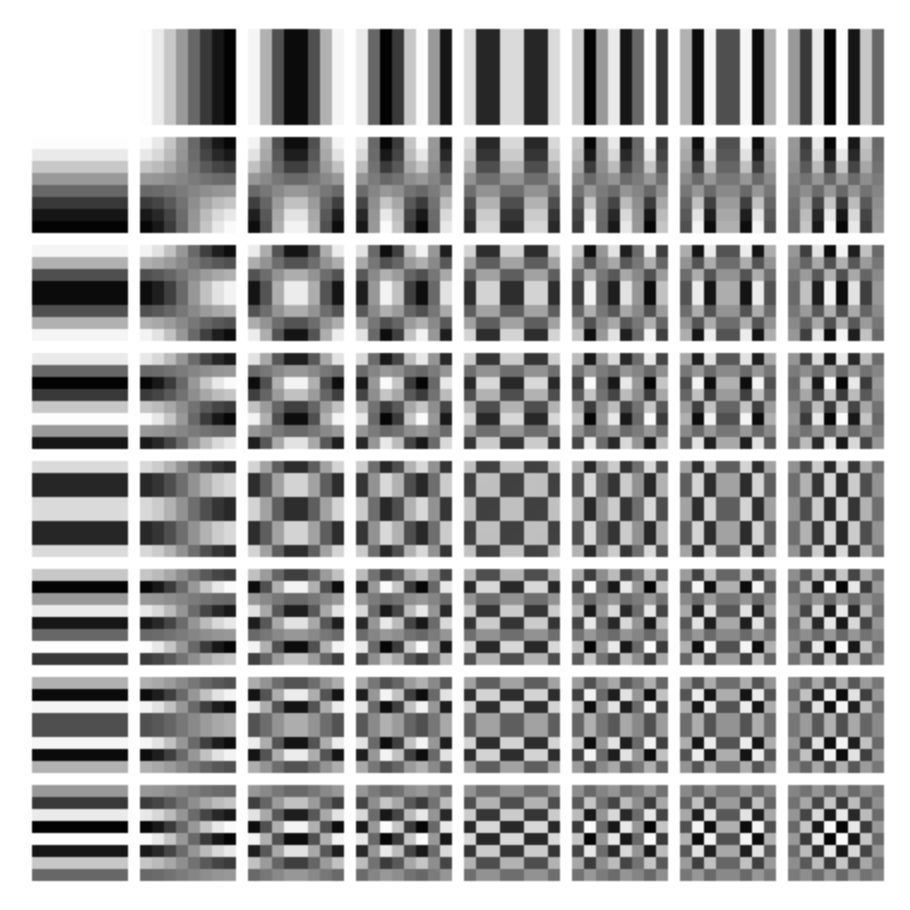
\includegraphics[width=\textwidth]{Pictures/DCT.png}
    \caption{DCT representation of an MCB. Each cell of the block here contains an image of the pattern it represents.}
    \label{fig:DCT}
    \end{minipage}
\hspace{0.05\linewidth}
    \begin{minipage}[b]{0.25\linewidth}
    \centering
    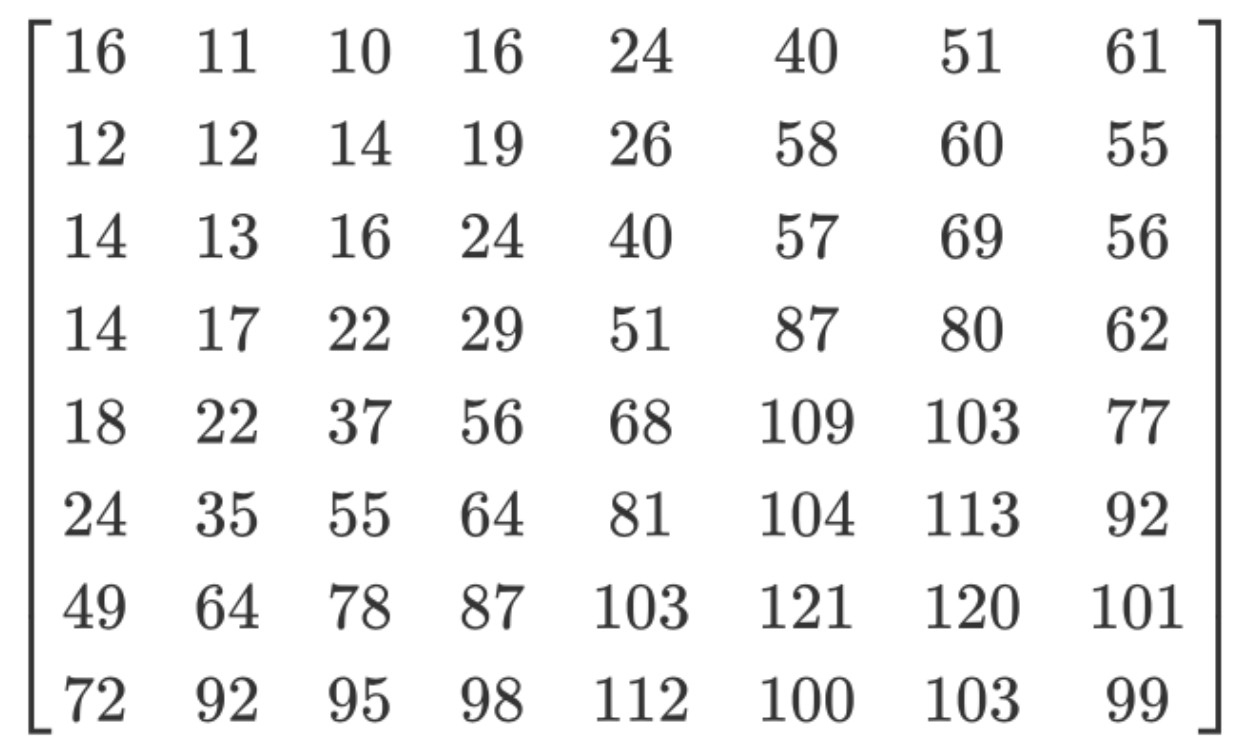
\includegraphics[width=\textwidth]{Pictures/quantization_table.png}
    \caption{Example Quantization Table. Every cell of a 8x8 frequency-domain block is divided by the value in the corresponding cell of the quantization table}
    \label{fig:quantizationTable}
    \end{minipage}
\hspace{0.05\linewidth}
    \begin{minipage}[b]{0.24\linewidth}
    \centering
    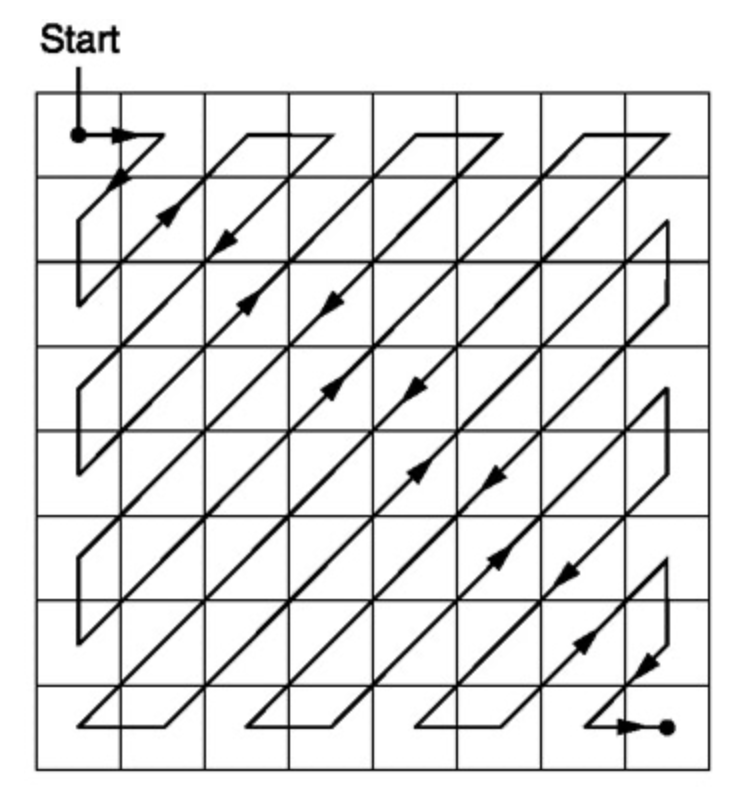
\includegraphics[width=\textwidth]{Pictures/ZigZag.png}
    \caption{Zig-Zag order for the serialization of the frequency-domain blocks}
    \label{fig:ZigZag}
    \end{minipage}
\end{figure}


%New colors defined below
\definecolor{codegreen}{rgb}{0,0.6,0}
\definecolor{codegray}{rgb}{0.5,0.5,0.5}
\definecolor{codepurple}{rgb}{0.58,0,0.82}
\definecolor{backcolour}{rgb}{0.95,0.95,0.92}

%Code listing style named "mystyle"
\lstdefinestyle{mystyle}{
  backgroundcolor=\color{backcolour},   commentstyle=\color{codegreen},
  keywordstyle=\color{magenta},
  numberstyle=\tiny\color{codegray},
  stringstyle=\color{codepurple},
  basicstyle=\ttfamily\footnotesize,
  breakatwhitespace=false,
  breaklines=true,
  captionpos=b,
  keepspaces=true,
  numbers=left,
  numbersep=5pt,
  showspaces=false,
  showstringspaces=false,
  showtabs=false,
  tabsize=2
}

%"mystyle" code listing set
\lstset{style=mystyle}

\chapter{Implementation} \label{implementation}

\section{Encoding algorithm}
The original NanoJPEG library, written in C, has an API composed of two main functions: \texttt{njDecode()}, which receives raw JPEG data in a byte array and does the actual decoding, and \texttt{njGetImage()}, which copies the decoded image from an internal buffer back to the caller. The whole library uses a static state structure, so it is not thread-safe, however passing the state structure as parameter would allow multithreading.

% \begin{lstlisting}
% bool writeJpeg(WRITE_ONE_BYTE output, const void* pixels_, unsigned short width, unsigned short height, bool isRGB, unsigned char quality_, bool downsample, const char* comment)
% \end{lstlisting}
% It accepts, in order:
% \begin{itemize}
%     \item the output writer buffer;
%     \item the pixels of the image;
%     \item width and height dimensions;
%     \item a flag to select if it is RGB or grayscale;
%     \item a value between 0 and 100 for the quality;
%     \item a downsample flag to select if use YCbCr 4:4:4 or 4:2:0;
%     \item a comment for the JFIF header. 
% \end{itemize}

Decompressing a JPEG image is simpler than creating it for three reasons: the input size is already known (the output size is fixed by width and height), there is no quality setting (the quantization table is already known), and there are no choices to be made about the compression (the Huffman table us already known).\\
Decompressing JPEG images could also be complicated by the myriad legal combinations of color spaces and representation formats and advanced features. NanoJPEG deals with this complexity by supporting only a core set of features, that in practice cover most use cases: only a few color spaces (YCbCr, RGB and single channel) are supported with any integer subsampling ratio on any channel, and no progressive scan (which is the most immediate limit of the library).

Although the order in which the specific functions are called is slightly different, the data flow can be summarized as:
\begin{itemize}
    \item Read 8x8 data blocks from stream
    \begin{itemize}
        \item Read DC differential coefficient and compute DC coefficient (sum of last DC coef and difference)
        \item Read Huffman Variable Length Codes until end of block (function \texttt{njGetVLC()})
        \item Convert from Huffman code to numeric value using the correct code for the component
        \item De-quantize or rescale AC coefficients: multiply each by the corresponding value in the correct Quantization Table for the component
    \end{itemize}
    \item Inverse Discrete Cosine Transform (IDCT) (functions \texttt{njRowIDCT()} and \texttt{njColIDCT()})
    \item rescaling of components which are downsampled (functions \texttt{njUpsampleH()} and \texttt{njUpsampleV()} called inside \texttt{njConvert()})
    \item Convert to RGB color space if different (inside function \texttt{njConvert()})
    \item Copy back to user buffer (separate user API call, function \texttt{njGetImage()})
\end{itemize}
Of these phases, the read and write phases cannot be processed on a GPGPU because they are inherently serial.\\
The other phases can exploit parallel computing since any pixel depends at most from a few neighboring pixels.

\section{NanoJPEG CUDA Implementation Details}

NanoJPEG CUDA compiles with the standard \texttt{nvcc} compiler.\\
The library allows the user of the API to disable all CUDA features, by setting to zero the parameter \texttt{use\_cuda} of function \texttt{njInit()}.

The block diagram of the CUDA version of the library is shown in \autoref{fig:nanojpeg_diag}.
\begin{figure}[h]
    \centering
    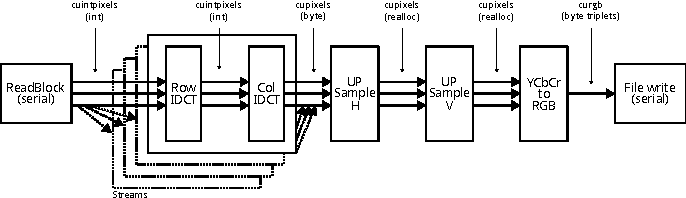
\includegraphics[width=1\textwidth]{Pictures/flow01.pdf}
    \caption{Data flow of NanoJPEG CUDA}
    \label{fig:nanojpeg_diag}
\end{figure}

NanoJPEG CUDA is divided into two main parts: function \texttt{\textbf{njCudaDecodeScan()}} handles from input data up to the IDCT, while function \texttt{\textbf{njCudaConvert()}} handles upsampling and RGB color space conversion.

Read from stream, Huffman decoding and de-quantization are implemented in function \texttt{njReadBlock()}, which is CPU-only.

The bi-dimensional IDCT is implemented as two separate functions, \texttt{njCudaRowIDCT()} and \texttt{njCudaRowIDCT()}.

The image is divided into four horizontal slices. When \texttt{njReadBlock()} finishes reading one slice, \texttt{njCudaRowIDCT()} and \texttt{njCudaRowIDCT()} are executed for that slice. The IDCTs for the four slices are executed in four separate CUDA streams so that an initial \texttt{CudaMemcpyAsync()} and the IDCT kernels can run on the GPU while the CPU reads the next slice from file. As a result, the starting times of the IDCTs in the four streams are staggered. This allows to reduce non-parallelizable task time at the beginning of the algorithm, since only a quarter of the file needs to be read before the GPU can start.

The program is disk-bound anyway, so a lower number of threads (as low as 2) could in theory be used, alternating the execution of the IDCT kernels between the first and the second, optionally subdividing the IDCT task in more than 4 slices. However the speed gain would be very small, most probably negated by the kernel setup time. Also, the creation of streams is comparatively cheap, so the solution using four streams was chosen.\\
\autoref{fig:streams} shows the sequence of kernel executions.

\begin{figure}
    \centering
    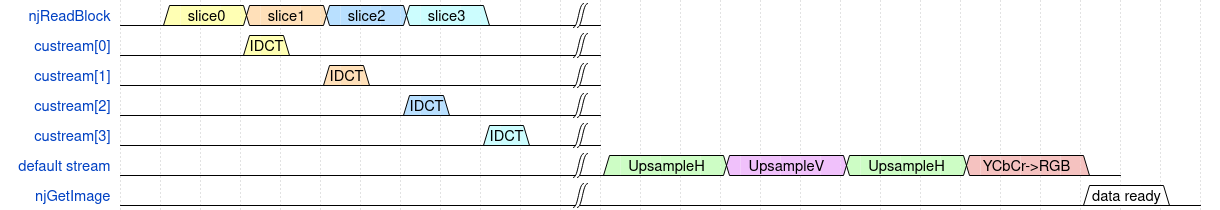
\includegraphics[width=1\textwidth]{Pictures/wavedrom_sequenza.png}
    \caption{Execution timeline}
    \label{fig:streams}
\end{figure}

Upsampling is optional, depending on the content of the file. In general functions \texttt{njCudaUpsampleH()} and \texttt{njCudaUpsampleV()} can be executed many times on any component, each doubles the size of the image in the horizontal or vertical axis respectively.

Eventually the image is converted back to the RGB format, which is a simple linear function implemented in integer arithmetic.

\section{Test application nanoex.cu}
The test application provided with the library (\texttt{nanoex.cu}) simply reads a JPEG file, decodes it using NanoJPEG, and writes the uncompressed result to a PPM file.

The test program received minor modifications to test NanoJPEG CUDA.

A new command-line option \texttt{"-nocuda"} was added to test the non-CUDA version of the library.
\chapter{Results and Conclusions} \label{results}

The execution time of the original and modified libraries were compared on an NVidia Jetson Nano ARM board. As was already observed by Simone Pistilli in \cite{simonepap} for the JPEG compression algorithm, NanoJPEG CUDA also shows better performance than the original NanoJPEG only above a certain image size, which is roughly 1 Megapixel, YCbCr 4:2:0.

YCbCr 4:4:4 moves the convenience threashold higher, because no upsampling is needed, reducing the opportunities to use GPU time.

Halving of the processing time was observed on a 6000x4000 image on the CUDA version compred to the original.

The process is substantially bound by the disk I/O bandwidth. Using four streams for IDCT allows to copy data to the GPU and to execute the IDCT kernels while the CPU is still reading data from disk, reducing serial time of the operation. The reduction is however far smaller than the theoretical 75\% because in this phase of the algorithm the GPU is under-utilized. An intermediate version of the program with a single CUDA stream for the IDCT showed a time penalty of 23\% compared to the final version with four streams (image: 4272x2848 YCbCr 4:2:0 shown in much smaller form in \autoref{fig:foresta}).

The image size lower threshold discourages the use of this library for consumer products, however future applications could arise that would benefit from the use of dedicated processing power to decompress very high resolution images in real-time, embedded applications, in which case the use of GPGPUs for the purpose would be second only to application specific processors.

\begin{figure}
    \centering
    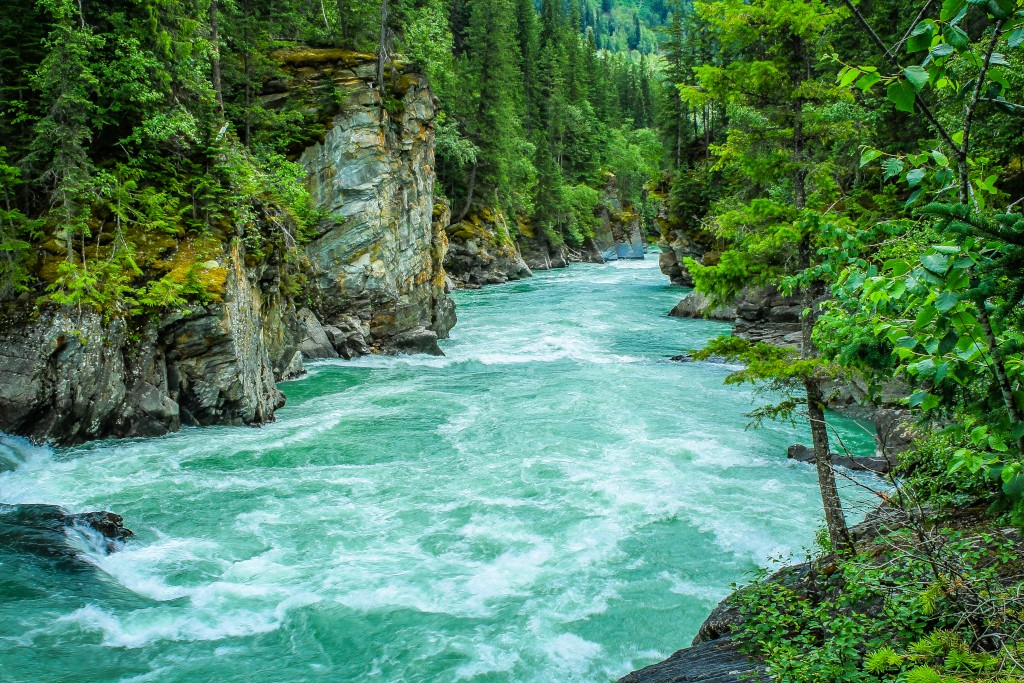
\includegraphics[width=1\textwidth]{Pictures/ph1_small.jpg}
    \caption{Thumbnail of a 4272x2848 pixel, YCbCr 4:2:0 image which in the decompression tests showed a speedup from 3.5s (with the original NanoJPEG), to 2.7s (with one-stream NanoJPEG CUDA), to 2.23s (with final NanoJPEG CUDA)}
    \label{fig:foresta}
\end{figure}

%\input{./chapters/conclusions.tex}         %included in results



\bibliography{references}

\appendix

\end{document}

